\documentclass[a4paper]{article}
\usepackage{problemsheet_mathsim}
\usepackage{pythontex} 
\usepackage{setspace}
\usepackage{graphicx}


\begin{document}
% \include{draft_sheet}
\include{sheet1}
%%%%%%%%%%%%%%%%%%%%%%%%%%%%%%%%%%%%%%
% Numerical Linear Algebra class 2022 
% Solutions to Sheet 1
%%%%%%%%%%%%%%%%%%%%%%%%%%%%%%%%%%%%%%

\begin{SolutionSheet}[\ref{sheet1}]

  \begin{Solution}
    \begin{itemize}
      \item \textit{Def projection:} Let $V$ be a vectorspace (VS). \\
        A linear map $P: V \to V$ is called projection $\ \iff \ P^2 = P$
      \item \textit{Def orthogonal projection:} Let $V$ be a VS, $W \subseteq V$ a subspace 
        and $\langle \cdot \; , \; \cdot \rangle$ be an inner product on V. \\
        $P_w$ is called orthogonal projection $\ \iff \ P_w$ is a projection and 
        $P_w(v)-v \bot W \quad \forall v\in V$
      \item \textit{Theorem:} Orthogonal projection is uniquely determined by the subspace \\
        \textit{Proof:} Existance: Gram Schmidt \\
        Uniqueness: Let $V$ finite dim VS with inner product $\langle \cdot \; , \; \cdot \rangle$,
        $W \subseteq V$ subspace, $P_w$ and $P_w'$ two orthogonal projections on $W$. \\
        $\implies P_w(v)-v \bot W \forall v \in V$ 
        \begin{align*}
          \langle P_w(v) - P_w'(v), w \rangle &= \langle (P_w(v) - v) - (P_w(v) - v), w \rangle \\
          &= \langle P_w(v) - v , w \rangle - \langle P_w'(v) - v , w \rangle \\
          &= 0 - 0 \ = \ 0 \quad \forall v\in V, \ \forall w\in W
        \end{align*}
        $\implies P_w(v) - P_w'(v) = 0 \quad \forall v \in V$ \\
        $\implies P_w = P_w'$
      \item \textit{Theorem (Best Approximation):} Let $W \subseteq \mathbb{R}^n$ subspace,
        $\widetilde{x}$ the orthogonal projection of $x \in \mathbb{R}^n$ in $W$ \\
        $\implies \norm{x - \widetilde{x}} \leqslant \norm{x - w} \forall w \in W$ \\
        \textit{Proof:}  
        \begin{align*}
          \norm{x - w}^2 = & \norm{(x - \widetilde{x}) + (\widetilde{x} - w)}^2 \\
          \stackrel{\text{Pythagoras}}{=} & \norm{(x - \widetilde{x})} + \norm{(\widetilde{x} - w)}^2
          \leqslant \norm{(\widetilde{x} - w)}^2
        \end{align*}
      \item \textit{Theorem:} Orthogonal projection in orthonormal basis \\
        \textit{Proof:} Just compute and see $P_w$ is an orthogonal projection
      \item \textit{Theorem (Parseval identity):} Let $V$ VS, $\{e_1, ... ,e_n\}$ an orthogonal basis. 
        Then $\forall x \in V :$ 
        \begin{equation}
          x = \sum\langle x, e_i \rangle e_i
        \end{equation}
        \textit{Proof:}
        $x = \sum a_i e_i \\
        \implies \langle x , e_j \rangle = \sum a_i \langle e_i, e_j \rangle = a_j \\
        \implies x = \sum \langle x, e_i \rangle e_i \\
        \implies \norm{x}^2 = \langle x,x \rangle = \langle\sum \langle
          a,e_i\rangle e_i,\sum \langle a,e_j\rangle e_j \rangle \\
        \phantom{\implies \norm{x}^2 = \langle x,x \rangle} = \sum \sum \langle x, e_i \rangle\langle x,e_j \rangle\langle e_i,e_j \rangle \\
        \phantom{\implies \norm{x}^2 = \langle x,x \rangle} = \sum | \langle x, e_i \rangle |^2$
    \end{itemize}
  \end{Solution}

  \begin{Solution}
    \textit{Claim:} Every finite-dim VS with a scalar product has an orthonormal basis.\\
    \textit{Proof:} Use Gram-Schmidt on any basis of the VS.
  \end{Solution}

  \begin{Solution}
    Let $M=\big(\begin{smallmatrix}
      c & s\\
      -s & c
    \end{smallmatrix}\big) \in \mathbb{R}^{2\times 2} \quad$ with $c = cos(\alpha), \ s = sin(\alpha), \ \alpha \in \mathbb{R}$ \\
    \begin{itemize}
      \item \textit{Eigenvalues:} $0 = det(M-\lambda I) = \lambda^2 - 2c\lambda + 1 \\
        \implies \lambda_{1,2} \ = \ c \pm is \ = \ e^{\pm i\alpha}$ \\
      \item \textit{Eigenvectors:} $(M-\lambda I)x = 0 \\
        \lambda_1 = e^{i\alpha}: \quad x_1 = \alpha \big(\begin{smallmatrix}
          1\\
          i
        \end{smallmatrix} \big)\\
        Eig(\lambda_1) = span\{x_1\}
        \lambda_2 = e^{-i\alpha}: \quad x_2 = \alpha \big(\begin{smallmatrix}
          1\\
          -i
        \end{smallmatrix} \big)\\
        Eig(\lambda_2) = span\{x_2\}$
      \item $\alpha \in \pi \mathbb{Z} \ \implies \ M=\big(\begin{smallmatrix}
          \pm 1 & 0\\
          0 & \pm 1
        \end{smallmatrix}\big) \\
        \implies \lambda_{1,2} = \pm 1, \ Eig(\lambda_{1,2}) = \mathbb{C}^2$
    \end{itemize}
  \end{Solution}

  \begin{Solution}[Programming]
  \end{Solution}

\end{SolutionSheet}


%%% Local Variables: 
%%% mode: latex
%%% TeX-master: "main"
%%% End: 

\include{sheet2}
%%%%%%%%%%%%%%%%%%%%%%%%%%%%%%%%%%%%%%
% Numerical Linear Algebra class 2022 
% Solutions to Sheet 2
%%%%%%%%%%%%%%%%%%%%%%%%%%%%%%%%%%%%%%



\begin{SolutionSheet}[\ref{sheet2}]
\begin{onehalfspace}

  \begin{Solution}
    \Claim $A$ normal $\ \iff A = Q^{-1}BQ \ $ with $Q$ unitary, $B$ normal
    \Claim $"\implies ": \ A$ is normal, $A \sim A$ \\
    $"\Leftarrow ":$ Let $A$ be a unitarily similar to $B$, $B$ normal \\
    $ \implies BB^* = B^*B, \quad\exists Q \in U(n): A = Q^{-1}BQ$ \\
    $ \implies$ \begin{align*}
      AA^* &= Q^{-1}BQ(Q^{-1}BQ)^* \\
      &= Q^{-1}BQ Q^* B^* (Q^{-1})^* \\
      &= Q^{-1} BB^*Q \\
      &= Q^{-1} B^*BQ \\
      &= Q^{-1} B^* QQ^{-1}BQ \\
      &= (Q^* B^* Q)(Q^{-1}BQ) \\
      &= (Q^* B Q)^* A \\
      &= A^* A
    \end{align*}
    $ \implies A$ normal
  \end{Solution}

  \begin{Solution}
    \Claim $A$ normal, $Av = \lambda v \ 
      \implies \ v^* A = \lambda v^*$ \\
    \Proof Let $A$ be a normal matrix. \\
    $ $ note: \begin{equation*}
      \begin{split}
        \norm{Ax} = 0 \ &\iff \ \norm{Ax}^2 = 0 \quad 
          \iff \ \langle Ax,Ax \rangle = 0 \\
          &\iff \ \langle x, A^*Ax \rangle = 0 \ 
          \iff \ \langle x, AA^*x \rangle = 0 \\
          &\iff \  \langle A^*x,A^*x\rangle = 0 \: 
          \iff \ \norm{A^*x}^2 = 0 \\
          &\iff \ \norm{A^*x} = 0
      \end{split}
    \end{equation*}
    $\implies$ \begin{equation*}
      (A - \lambda \mathbb{I})^* 
        = (\overline{\rm A} - \overline{\rm \lambda \I})^T 
        = (A^* - \overline{\lambda} \I) 
    \end{equation*}
    $ \implies$ \begin{align*} 
      (A - \lambda \I)(A - \lambda \I)^* &= (A - \lambda \I)(A^* - \overline{\lambda} \I) \\
      &= AA^* - \lambda A^*\I - \overline{\lambda} A \I - \lambda \overline{\lambda} \I \\
      &= A^*A - \overline{\lambda} A \I - \lambda A^*\I - \lambda \overline{\lambda} \I \\
      &= (A^* - \overline{\lambda} \I)(A - \lambda \I) \\
      &= (A - \lambda \I)^* (A - \lambda \I)
    \end{align*}
    $ \implies A - \lambda \I$ is normal\\
    \\
    Let $v$ be a (right) eigenvector to $\lambda$ \\
    $\begin{array}{ll}      
      \implies &(A- \lambda \I)v = 0 \\
      \implies &(A- \lambda \I)^*v = 0 \\
      \implies &A^*v = \overline{\lambda} \I v \\
      \implies &v^T(A^*)^T = \overline{\lambda} v^T \\
      \implies &v^T \overline{A} = \overline{\lambda} v^T \\
      \implies &v*A = \lambda v^*
    \end{array}$

  \end{Solution}

  \begin{Solution} 
    $M = $ \smatrix{\eta}{1}{\eta}{\eta} with $|\eta| << 1 \\
    \begin{array}{ll}
      \implies & \lambda_{1,2}(M) = \eta \pm \sqrt{\eta}, \quad v_1 =$ \svector{\sqrt{\pm\eta}}{1} $\\
      \implies & v_1 \text{almost parralel to} v_2 
    \end{array}$
    
    Take \begin{equation*} \widetilde{M} := M + \Delta M \end{equation*}
    so $\widetilde{M}$ is a small change to $M$. \\
    \\
    $\begin{array}{lll} 
      e.g. &\Delta M = -(\eta)$ \smatrix{1}{0}{1}{1}$ \\
      &\implies \widetilde{M} =$ \smatrix{0}{1}{0}{0}$ \\
      &\implies \lambda_{1,2}(\widetilde{M}) = 0, \
      &v_{1,2}(\widetilde{M}) =$ \svector{1}{0} $\implies \text{not conituous}
    \end{array}$
  \end{Solution}

  \begin{Solution} \phantom{A}\\
    \begin{equation*}
      A =\begin{pmatrix} \cos\phi & -\sin\phi\\
        \sin\phi &  \cos\phi  \end{pmatrix}^T
      \begin{pmatrix}  1 & \\
          & c \end{pmatrix}
      \begin{pmatrix} \cos\phi & -\sin\phi\\
        \sin\phi &  \cos\phi \end{pmatrix} =: R^T A R
      \end{equation*}
    \begin{enumerate}
      \item $R$ orthogonal \\
        $\stackrel{\text{Lemma 1.1.13}}{\implies} A$ diagonalizable, $R$ orthogonal basis of eigenvectors \\
        $\implies \lambda_1 = 1, \ \lambda_2 = c, \quad
        v_1 =$ \svector{\cos\phi}{\sin\phi}, $\ v_2 =$ \svector{-\sin\phi}{\cos\phi}
      \item (Programming)
      \item $c=1 \ \implies \ A = \I \ \implies \ x^{(i)} = x^{(0)} \ \forall i$. \\
        Since $A^n$ converges (see (4)), $A^nx$ converges, too.
      \item $\begin{array}{ll}
        lim_{n \to \infty} A^n &\stackrel{\text{R orthogonal}}{=} R^T \: lim_{n \to \infty}$ \smatrix{1}{}{}{c} $R \\
        &= R^T$ \smatrix{1}{}{}{0} $R \\
        &=$ \smatrix{(\cos\phi)^2}{-\sin\phi\cos\phi}{-\sin\phi\cos\phi}{(\sin\phi)^2} $
      \end{array}$
    \end{enumerate}
  \end{Solution}

\end{onehalfspace}
\end{SolutionSheet}


%%% Local Variables: 
%%% mode: latex
%%% TeX-master: "main"
%%% End: 

\include{sheet3}
%%%%%%%%%%%%%%%%%%%%%%%%%%%%%%%%%%%%%%
% Numerical Linear Algebra class 2022 
% Solutions to Sheet 3
%%%%%%%%%%%%%%%%%%%%%%%%%%%%%%%%%%%%%%

\begin{SolutionSheet}[\ref{sheet3}]
  \begin{onehalfspace}
    

  \begin{Solution} $A \in \C^{n\x n}$ hermitian, $ \ Q: \C^m \to \C^n \ (m<n) \ $ unitary, linear \\
    $B = Q^*AQ \in \C^{m \x m}$ \\
    \\
    \Claim $\forall\lambda_k \in\sigma(B): \quad \lambda_k =0$ or \begin{equation*}
        |\lambda_{min}(A)| \leq |\lambda_k (B)| \leq |\lambda_{max}(A)|
      \end{equation*}
    \Proof Let $v\in \C^m, v\neq 0.$ \\
    \\
    $\begin{array}{lll}
     \implies & \lambda_{max}(B) &\stackrel{\textit{Courant Fischer}}{=} \ \max_{v\in \C^m} \frac{v^*Bv}{v^*v} \\
      &&= \max_{v\in \C^m} \frac{v^*Q^*AQv}{v^*v} \\
      &&= \max_{w \in range(Q)} \frac{w^*Aw}{w^*(Q^*)^{-1}Q^{-1}w} \\
      && \leq \max_{w\in \C^n} \frac{w^*Aw}{w^*w} \\
      &&\stackrel{\textit{Courant Fischer}}{=} \lambda_{max}(A)
    \end{array}\\
    \\
    \implies |\lambda_k(B)| \leq |\lambda_{max}(A)| \quad \forall k = 1,...,n$\\
    (Other estimate analogous to max.)
  \end{Solution}

  \begin{Solution}
    $A$ diagonizable, real \\
    $\sigma(A) = \{-2, \ 1-2i, \ 1+2i, \ 1, \ -i, \ i, \ 2\}$ \\
    The power method converges to $\lambda\in \sigma(A)$ such that \begin{equation*}
      |\lambda - \sigma| = max
    \end{equation*} 
    $\implies $ does not converge for \begin{equation*}
      max = |\lambda_i -\sigma| = |\lambda_j - \sigma| \qquad (\lambda_i \neq \lambda_j)
    \end{equation*} 
    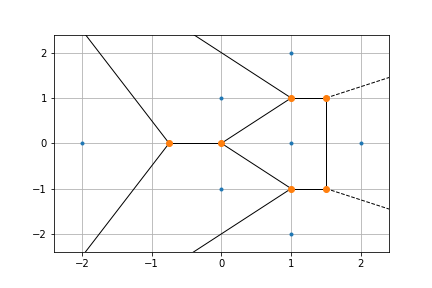
\includegraphics[width=7cm]{include/sheet3_ex2.png}\\
    (b) Wikipedia: \begin{equation*}
      \text{error} = \mathcal{O}\big(\frac{|\mu -\lambda_1|}{|\mu -\lambda_2|}\big) 
    \end{equation*}
    where $\lambda_1$ is the eigenvalue closest to $\sigma$, $\lambda_2$ the second closest.\\
    \\
    To find $\lambda = 2$:\\
    $\begin{array}{ll}
      \sigma > 2 &\implies \frac{1}{10} \geq \frac{\sigma - 2}{\sigma - 1}\\
        &\iff \frac{1}{10}\sigma - \frac{1}{10} \geq \sigma - 2 \\
        &\iff 2-\frac{1}{10} \geq \frac{9}{10}\sigma \\
        &\iff \frac{19}{9} \geq \sigma \\
        \\
      1 < \sigma < 2 &\implies \frac{1}{10} \geq \frac{2-\sigma}{\sigma -1} \\
       &\iff \frac{1}{10}\sigma - \frac{1}{10} \geq 2-\sigma \\
       &\iff \frac{11}{10}\sigma \geq \frac{21}{10} \\
       &\iff \sigma \geq \frac{21}{10}
    \end{array}\\
    \implies \text{ for }  \lambda=2  \text{ choose shift } \sigma\in  [\frac{21}{11}, \frac{19}{9}] $
  \end{Solution}

  \begin{Solution} Find shift parameters for $A= \begin{pmatrix}
    100 & 15 & 3 \\
    15 & 20 & 5 \\
    3 & 5 & 65
  \end{pmatrix}$\\
  Use Gershgorin Circle Theorem to obtain the circles: \\
  $D_1(100,18), \ D_2(20,20), \ D_3(65,8) \quad$ \\
  i.e. the intervals: $I_1[92,118], \ I_2[0,40], \ I_3[57,73]$\\
  The intervals are distinct $ \ \implies \ $ there is exactly one eigenvalue in each interval \\
  $\implies$ choose centers of intervals as shifts 
  \end{Solution}

  \begin{Solution}[Programming]
  \end{Solution}

\end{onehalfspace}

\end{SolutionSheet}


%%% Local Variables: 
%%% mode: latex
%%% TeX-master: "main"
%%% End: 

%%%%%%%%%%%%%%%%%%%%%%%%%%%%%%%%%%%%%%
% Numerical Linear Algebra class 2022 
% Sheet 4
%%%%%%%%%%%%%%%%%%%%%%%%%%%%%%%%%%%%%%

\begin{Sheet}[to be handed in until November 18, 2022, 2pm.]
  \label{sheet4}

  \begin{Problem}
    Let $\mata$ be a symmetric tridiagonal matrix. Show that the
    QR-iteration (see Algorithm 1.4.3 in the lecture notes) preserves
    the tridiagonal structure of the matrix, i.e., all iterates
    $\mata^{(n)}$ generated by the QR-iteration are tridiagonal.
  \end{Problem}

  \begin{Problem}
    Show that a (complex) symmetric matrix can be transformed to a
    tridiagonal matrix by using similarity transformations (this
    proves Theorem 1.4.14 in the lecture notes).
    \begin{todo}
      Rewrite: Show, that if A symm, H in 1.4.16 is tridiagonal
    \end{todo}
  \end{Problem}

  \begin{Problem}
    Rewrite the QR factorization of a tridiagonal (complex) symmetric
    matrix such that its complexity is of order $O(n)$ (this proves
    the second part of Corollary 1.4.13 in the lecture notes).
  \end{Problem}

  \begin{Problem}
    Find an example of a matrix with a real spectrum for which the QR
    method will \textit{not} converge to an upper triangular matrix.
  \end{Problem}

  \begin{Problem}[Programming]
    \hfill\\\vspace{-6ex}
    \begin{enumerate}[(a)]
    \item Implement the Hessenberg QR step (Algorithm 1.4.12 in the
      lecture notes) in real arithmetic.
    \item Test your code with the tridiagonal matrix
      $\mata_n=\operatorname{tridiag}(-1.,2.,-1.)$ in dimension $n=4$
      and check, if your results are correct.
    \item Use your implementation to run several steps of the QR
      iteration (Algorithm 1.4.3 in the lecture notes) for the matrix
      $\mata_{10}$.
    \item Discuss the observed convergence of the off-diagonal and
      diagonal entries, respectively.
    \end{enumerate}
  \end{Problem}

\end{Sheet}


%%% Local Variables: 
%%% mode: latex
%%% TeX-master: "main"
%%% End: 

%%%%%%%%%%%%%%%%%%%%%%%%%%%%%%%%%%%%%%
% Numerical Linear Algebra class 2022 
% Solutions to Sheet 4
%%%%%%%%%%%%%%%%%%%%%%%%%%%%%%%%%%%%%%

\begin{SolutionSheet}[\ref{sheet4}]
\begin{onehalfspace}
  
  \begin{Solution}
    \Claim The QR-iteration preserves the tridiagonal structure of a symmetric tridiagonal matrix. \\
    \Proof We know for the QR-iteration $A_{k+1} = R_kQ_k$ and $A_k = Q_kR_k$ \\
      $\implies A_{k+1} = Q_k^*A_kQ_k \\
      \implies A_{k+1} = U_k^*A_0 U_k$ with $U_k = Q_1 \dot ... \dot Q_k \\
      \implies$ with $A_0$ is $A_{k+1}$ also hermitian: \begin{equation*}
        A_{k+1}^* = (U_k^*A_0 U_k)^T = U_k^T A_0^T (U_k^*)^T = 
        \overline{U_k^*} A_0 \overline{U_k} = \overline{A_{k+1}}
      \end{equation*}
      With Lemma B.1.2 we know: \begin{equation*}
        span{a_1,...,a_i} = span{q_1,...,q_i} \quad i=1,...,n
      \end{equation*}
      and $a_k = \sum_{i=1}^n r_{ik}q_i \\
      \\
      A_k = \begin{pmatrix}
        \ast & \ast &&& \\
        \ast & \ddots & \ddots &0& \\
        &\ddots&\ddots&\ddots&\\
        & 0 &\ddots & \ddots &\ast \\
        & & &\ast & \ast 
      \end{pmatrix} = \underbrace{\begin{pmatrix}
        \ast & & && \\
        \ast & \ddots && \ast& \\
        &\ddots& \ddots&&\\
        &0 & \ddots& \ddots\\
        & && \ast & \ast
      \end{pmatrix}}_{Q_k} \underbrace{\begin{pmatrix}
        \ast & \ast &\ast && 0 \\
        &\ddots&\ddots&\ddots& \\
        && \ddots & \ddots & \ast \\
        & 0 && \ddots &\ast \\
        & &&  & \ast
      \end{pmatrix}}_{R_k} \\
      \\
      \underbrace{\begin{pmatrix}
        \ast & \ast &\ast && 0 \\
        &\ddots&\ddots&\ddots& \\
        && \ddots & \ddots & \ast \\
        & 0 && \ddots &\ast \\
        & &&  & \ast
      \end{pmatrix}}_{R_k} \underbrace{\begin{pmatrix}
        \ast & & && \\
        \ast & \ddots && \ast& \\
        &\ddots& \ddots&&\\
        &0 & \ddots& \ddots\\
        & && \ast & \ast
      \end{pmatrix}}_{Q_k} = \begin{pmatrix}
        \ast & & && \\
        \ast & \ddots && \ast& \\
        &\ddots& \ddots&&\\
        &0 & \ddots& \ddots\\
        & && \ast & \ast
      \end{pmatrix} = A_{k+1}\\
      \\
      \stackrel{A_{k+1} \text{hermitian}}{\implies} A_{k+1}$ is tridiagonal
  \end{Solution}

  \begin{Solution}
    \Claim For a symmeric matrix $A$, in the proof of Theorem  1.4.16, $H$ would be tridiagonal \\
    \Proof Any matrix $A\in \C ^{n\x n}$ can be transformed into a hessenberg matrix
    using similarity transformations st $H=Q^TAQ$ (with householder reflections for example). When A is symmetric, $H$ is also 
    symmetric and therefore tridiagonal.  
  \end{Solution}

  \begin{Solution}
  \end{Solution}

  \begin{Solution}
  \end{Solution}

  \begin{Solution}[Programming]
    The eigenvalues of $\mata_n$ are
    \begin{gather*}
      \lambda_{n,j} = 4\sin^2\left(\frac{j\pi}{2n+2}\right)
    \end{gather*}
  https://math.stackexchange.com/questions/3875168/eigenvalues-of-a-tridiagonal-matrix-with-1-2-1-as-entries

  https://math.stackexchange.com/questions/177957/eigenvalues-of-tridiagonal-symmetric-matrix-with-diagonal-entries-2-and-subdiago?rq=1
  \end{Solution}

\end{onehalfspace}
\end{SolutionSheet}


%%% Local Variables: 
%%% mode: latex
%%% TeX-master: "main"
%%% End: 

%%%%%%%%%%%%%%%%%%%%%%%%%%%%%%%%%%%%%%
% Numerical Linear Algebra class 2022 
% Sheet 5
%%%%%%%%%%%%%%%%%%%%%%%%%%%%%%%%%%%%%%

\begin{Sheet}[to be handed in until November 25, 2022, 2pm.]
  \label{sheet5}

  \begin{Problem}
    Show that a normal triangular matrix is diagonal. \textit{Hint:}
    look at the norms of $\mata \ve_i$ and $\mata^*\ve_i$.
  \end{Problem}

  \begin{Problem}
    Prove that in case of a normal real matrix, for each complex
    eigenvalue pair there is a $2\times 2$ matrix with according
    invariant subspace.
    \begin{enumerate}[(a)]
    \item Show that complex eigenvalues of a real matrix come in
      complex conjugate pairs.
      \begin{todo}
        Show that complex eigenvalues and their associated
        eigenvectors of a real matrix come in complex conjugate
        pairs.

        Delete (b)
      \end{todo}
    \item Show that the eigenvectors are of the form $\vu\pm i\vv$.
    \item Choose real linear combinations of these vectors to obtain
      the $2\times 2$ block.
    \end{enumerate}
  \end{Problem}

  \begin{Problem}
    Provide the following steps of Lemma 1.5.11 in the lecture notes
    (explicit double shift).
    \begin{enumerate}[(a)]
    \item Show that $\matq_1\matq_2\matr_2\matr_1$ represents the QR
      factorization of a real matrix
      $\matm = (\matH - \sigma_1\id)(\matH - \sigma_2\id)$.
    \item Show that $\matq_1\matq_2$ is the orthogonal matrix that
      implements the similarity transformation of $\matH$ to obtain
      $\matH_2$.
      \begin{todo}
        Adjust this exercise according to tutorial notes of Laura
      \end{todo}
    \end{enumerate}
  \end{Problem}

  \begin{Problem}[Programming]
    Implement the symmetric QR step with implicit shift (Algorithm
    1.5.6 in lecture notes) for a symmetric, unreduced, tridiagonal
    matrix $\matt$ by observing the following steps:
    \begin{enumerate}[(a)]
    \item Store $\matt$ in two vectors, one for the diagonal, and one
      for the subdiagonal entries.
    \item Implement the Givens rotation $\matg_{12}$ and think about
      where to store the additional non-zero entry $t_{31}$.
    \item Implement the additional Givens rotations for this data
      structure.
    \item Use this to compute the eigenvalues of the matrix
      $\mata_n=\operatorname{tridiag}(-1.,2.,-1.)$ in dimension
      $n=10$.
    \end{enumerate}
  \end{Problem}

\end{Sheet}


%%% Local Variables: 
%%% mode: latex
%%% TeX-master: "main"
%%% End: 

%%%%%%%%%%%%%%%%%%%%%%%%%%%%%%%%%%%%%%
% Numerical Linear Algebra class 2022 
% Solutions to Sheet 5
%%%%%%%%%%%%%%%%%%%%%%%%%%%%%%%%%%%%%%

\begin{SolutionSheet}[\ref{sheet5}]

  \begin{Solution}
    \Claim $A$ normal, triangular $\implies A$ diagonal \\
    \Proof Note \textit{(1)}: \begin{align*}
        \norm{Ae_i}^2 &= \langle Ae_i, Ae_i \rangle \\
        &= \langle e_i, A^*Ae_i \\
        &\stackrel{A \text{normal}}{=} \langle e_i, AA^* e_i \rangle \\
        &= \langle A^*e_i , A^*e_i \rangle \\
        &= \norm{A^*e_i}
      \end{align*}
      WLOG: $A$ upper triangluar.\\
      $\implies$ \begin{equation*}
        | a_{11} |^2 \quad \stackrel{\text{upper triang.}}{=} \quad \norm{Ae_1}^2 \
        \stackrel{\textit{(1)}}{=} \ \norm{A^*e_1} \ = \ \sum_{i=1}^{n} | a_{1i} |^2
      \end{equation*}
      $\implies \sum_{i=2}^{n} | a_{1i}|^2 = 0 \\
      \implies a_{1i} = 0 \quad \forall i=2,...,n\\
      \longrightarrow$ continue with rest of $e_i$
  \end{Solution}

  \begin{Solution}
    (a)+(b) \Claim $\forall A \in \mathbb{R}^{n\times n}$ every complex eigenvalue and their 
    corresponding eigenvectors come in complex conjugate pairs. \\
    \\
    \Proof Let $v$ be an eigenvector to an eigenvalue $\lambda$ of $A$.\\
    $\implies Av = \lambda v \\
    \implies A \overline{v} \stackrel{A \text{ real}}{=} \overline{Av} = \overline{\lambda} \overline{v} \\
    \implies (\overline{\lambda}, \overline{v})$ is eigenpair of $A$. \\
    \\
    (c) \Claim for each complex eigenvalue pair, there is a $2\times 2$ matrix with according invariant subspace.\\
    \Proof Let $\lambda=a+bi$ be an eigenvalue of $A$ with corresponding eigenvector $v= x+iy$ \\
    $\implies \lambda v = ax+iay+ibx-by = (ax-by) + i(bx+ay)$ \\
    and  $Av = Ax + iAy$ \\
    $\implies Ax = ax-by, \quad Ay = ab+ay$ \\
    Choose matrix \smatrix{a}{-b}{b}{a}: \\
    \\
    $\implies$ \smatrix{a}{-b}{b}{a} \svector{x}{y} = \svector{Ax}{Ay}
  \end{Solution}

  \begin{Solution} (a) \Claim $M := (H_0 - \sigma_1 \I)(H_0 - \sigma_2 \I) \stackrel{QR-fact}{=} Q_1Q_2R_2R_1$ \\
     where $H_0 - \sigma_1 \I = Q_1R_1 \ $ and $ \ H_1 - \sigma_2 \I = Q_2R_2$ \\
    \Proof \begin{align}
      H_0 - \sigma_1 \I &= Q_1R_1 \\
      H_1 &= R_1Q_1 + \sigma_1 \I \\
      H_1 - \sigma_2 \I &= Q_2R_2 \\
      H_2 &= R_2Q_2 + \sigma_2 \I
    \end{align}
    $\implies$ \begin{align*}
      Q_1Q_2R_2R_1 &\stackrel{\textit{(4)}}{=} Q_1(H_1 - \sigma_2 \I)R_1 \\
      &\stackrel{\textit{(3)}}{=} Q_1((R_1Q_1 + \sigma_1) - \sigma_2 \I)R_1 \\
      &= Q_1(R_1Q_1 + (\sigma_1 - \sigma_2) \I)R_1 \\
      &= Q_1R_1Q_1R_1 + (\sigma_1 - \sigma_2)Q_1R_1 \\
      &= Q_1R_1(Q_1R_1 + (\sigma_1 - \sigma_2)\I) \\
      &\stackrel{\textit{(2)}}{=} (H_0 - \sigma_1 \I)((H_0 - \sigma_1 \I) + (\sigma_1 - \sigma_2)\I) \\
      &= (H_0 - \sigma_1 \I)(H_0 - \sigma_2 \I) \quad = \quad M 
    \end{align*}
    and $Q_1, Q_2$ orthogonal $\implies Q_1Q_2$ orthogonal\\
    $\stackrel{\text{QR fact unique}}{\implies} Q_1Q_2R_2R_1$ is QR factorization of $M$. \\
    \\
    (b) \Claim $(Q_1Q_2)^* H_0 (Q_1Q_2) = H_2$ \\
    \Proof \begin{align*}
      (Q_1Q_2)^* H_0 (Q_1Q_2) &= Q_2^* Q_1^* H_1 Q_1Q_2 \\
      &\stackrel{\textit{(2)}}{=} Q_2^*Q_1^*(Q_1R_1 + \sigma_1 \I)Q_1Q_2 \\
      &= Q_2^*R_1Q_1Q_2 + \sigma_1 \I \\
      & \stackrel{\textit{(3)}}{=} Q_2^*(H_1 - \sigma_1 \I)Q_2 + \sigma_1 \I \\
      &= Q_2^*H_1Q_2 - \sigma_1 \I + \sigma_1 \I \\
      & \stackrel{\textit{(4)}}{=} Q_2^* (Q_2R_2 + \sigma_2 \I)Q_2 \\
      &= R_2Q_2 + \sigma_2 \I \\
      & \stackrel{\textit{(5)}}{=} H_2
    \end{align*}
  \end{Solution}

  \begin{Solution}[Programming]
  \end{Solution}

\end{SolutionSheet}


%%% Local Variables: 
%%% mode: latex
%%% TeX-master: "main"
%%% End: 

%%%%%%%%%%%%%%%%%%%%%%%%%%%%%%%%%%%%%%
% Numerical Linear Algebra class 2022 
% Sheet 6
%%%%%%%%%%%%%%%%%%%%%%%%%%%%%%%%%%%%%%

\begin{Sheet}[to be handed in until December 2, 2022, 2pm.]
  \label{sheet6}

  \begin{Problem}
    Prove that a matrix iteration converges \textit{if and only if}
    the spectral radius of the iteration matrix is less than 1.
    \textit{Hint:} You can use Lemma 2.2.10 in the lecture notes.
  \end{Problem}

  \begin{Problem}
    \label{sheet6:problem2}
    Consider the $n\times n$ tridiagonal matrix
    \begin{gather*}
      \matt_{\alpha} =
      \begin{pmatrix}
        \alpha &     -1 &        &        & \\
            -1 & \alpha &     -1 &        & \\
               & \ddots & \ddots & \ddots & \\
               &        &     -1 & \alpha &     -1 \\
               &        &        &     -1 & \alpha
      \end{pmatrix}
    \end{gather*}
    where $\alpha$ is a real parameter. Verify that the eigenvalues of
    $\matt_{\alpha}$ are given by
    \begin{gather*}
      \lambda_j = \alpha - 2\cos(j\theta),
    \end{gather*}
    where
    \begin{gather*}
      \theta = \frac\pi{n+1},
    \end{gather*}
    and the eigenvectors associated with each $\lambda_j$ are given by
    \begin{gather*}
      \vv_j = \left(
        \sin(j\theta),\ \sin(2j\theta),\ \ldots\ ,\ \sin(nj\theta)
      \right)^T.
    \end{gather*}
    What are the conditions on $\alpha$, such that the matrix
    $\matt_{\alpha}$ becomes positive-definite?
  \end{Problem}

  \begin{Problem}
    \label{sheet6:problem3}
    Let $\mata$ be a real symmetric positive-definite $n\times n$
    matrix and $\vb$ a vector in $\R^n$. Consider the Richardson
    iteration defined as
    \begin{gather*}
      \vx_{k+1}
      = \left(\id-\omega\mata \right)\vx_k + \omega\vb
      = \vx_k - \omega\left(\mata\vx_k - \vb \right)
    \end{gather*}
    where $\omega$ is a constant real parameter.
    \begin{enumerate}[(a)]
    \item Show that the sequence of iterates $\vx_k$ generated by the
      Richardson iteration converges to $\mata^{-1}\vb$ for any
      initial vector $\vx_0$ \textit{if and only if}
      \begin{gather*}
        0 < \omega < \frac{2}{\lambda_{\max}}.
      \end{gather*}
    \item Show that the optimal value of $\omega$ is
      \begin{gather*}
        \omega_{opt} = \frac2{\lambda_{\max} + \lambda_{\min}}.
      \end{gather*}
      Moreover
      \begin{gather*}
        \norm{\id-\omega_{opt}\mata}_2
        = \frac{\lambda_{\max} - \lambda_{\min}}{\lambda_{\max} + \lambda_{\min}}
        = \frac{\cond_2(\mata)-1}{\cond_2(\mata)+1},
      \end{gather*}
      where $\cond_2(\mata) = \frac{\lambda_{\max}}{\lambda_{\min}}$.
    \end{enumerate}
  \end{Problem}

  \begin{Problem}
    Apply the obtained results of Problem \ref{sheet6:problem3} to a
    one-dimensional Laplace problem. To this end, take matrix
    $\matt_{\alpha}$ from Problem \ref{sheet6:problem2} with
    $\alpha = 2$ and work on the following tasks.
    \begin{enumerate}[(a)]
    \item Will the Richardson iteration coverge for this matrix? If
      so, what will be its covergence rate?
      \begin{todo}
        How do you have to choose $\omega$, such that the Richardson
        iteration converges? What is the best choice?
      \end{todo}
    \item How many iterations are needed to reduce the error by a
      factor of $10^{-6}$ depending on the number $n$ of dicretization
      points?
    \item Estimate the cost of a single iteration (depending on $n$,
      use $\mathcal{O}(\cdot)$ notation).
    \item Estimate the cost of reducing the error by a given factor
      (depending on $n$, use $\mathcal{O}(\cdot)$ notation).
    \end{enumerate}
  \end{Problem}

\end{Sheet}


%%% Local Variables: 
%%% mode: latex
%%% TeX-master: "main"
%%% End: 

%%%%%%%%%%%%%%%%%%%%%%%%%%%%%%%%%%%%%%
% Numerical Linear Algebra class 2022 
% Solutions to Sheet 6
%%%%%%%%%%%%%%%%%%%%%%%%%%%%%%%%%%%%%%

\begin{SolutionSheet}[\ref{sheet6}]
\begin{onehalfspace}
  
  \begin{Solution}
    \Claim matrix it $x^{(k+1)} = Mx^{(k)} + g$ converges $\iff \rho(M) < 1$\\
    \Proof $"\implies":$ A linear iteration converges $\iff \quad M^k \conv{k} 0$ \\
    $\phantom{\implies}$ Let $\lambda$ be the largest eigenvalue and $v$ a normed corresponding eigenvector. \\
    $\phantom{\implies} \implies $\begin{equation*}
      0 \ = \ \lim_{k \to \infty} M^k v \ = \ \lim_{k \to \infty} \lambda^k v \ = \ v \lim_{k \to \infty} \lambda^k
    \end{equation*}
    $\phantom{\implies} \implies \lambda^k \conv{k} 0 \\
    \phantom{\implies} \implies |\lambda| < 1 \\
    \phantom{\implies} \stackrel{\text{def } \rho(M)}{\implies} \rho(M) < 1$\\
    \\
    $"\Longleftarrow": \rho(M) < 1 \\
    \phantom{\implies} \implies \exists \ \epsilon_0 > 0$, st $\ \rho(M)+\epsilon_0 < 1 \\
    \phantom{\implies} \stackrel{\text{2.2.12}}{\implies} \exists \ \norm{\cdot}_{M,\epsilon_0} =: \norm{\cdot}$, st \begin{equation*}
      \norm{M} \leq \rho(M) + \epsilon_0 < 1 
    \end{equation*}
    $\phantom{\implies} \implies$\begin{equation*}
      \norm{M^k} \leq \norm{M}^k \conv{k} 0
    \end{equation*}
    $\phantom{\implies} \stackrel{\norm{\cdot} \text{ continuous}}{\implies} M^k \conv{k} 0$
  \end{Solution}

  \begin{Solution} Varify eigenvalues and eigenvectors of $T_{\alpha}$: \\
    \begin{align*}
      T_{\alpha} q_j &=  \begin{pmatrix}
        \alpha &     -1 &        &        & \\
            -1 & \alpha &     -1 &        & \\
              & \ddots & \ddots & \ddots & \\
              &        &     -1 & \alpha &     -1 \\
              &        &        &     -1 & \alpha
      \end{pmatrix} \begin{pmatrix}
        sin(j\theta) \\ 
        \\
        \vdots\\
        \\
        sin(nj\theta)
      \end{pmatrix} \\
      &= \begin{pmatrix}
        \alpha sin(j\theta) - sin(2j \theta) \\
        -sin(j \theta) + \alpha sin(2j\theta) - sin(3j \theta)\\
        \vdots \\
        -sin((n-2)j \theta) + \alpha sin((n-1)j\theta) - sin(n j \theta)\\
        -sin((n-1)j \theta) + \alpha sin(n j \theta)\\
      \end{pmatrix} \\
      &= \begin{pmatrix}
        \alpha sin(j\theta) - sin(j\theta - j\theta) - sin(j\theta + j\theta) \\
        \\
        \vdots \\
        \\
        \alpha sin(nj\theta) - sin(nj\theta - j\theta) - sin(nj\theta + j\theta)
      \end{pmatrix} \\
      &= \begin{pmatrix}
        \alpha sin(j\theta) - 2 cos(j\theta)sin(j \theta) \\
        \\
        \vdots \\
        \\
        \alpha sin(nj \theta) - 2 cos(j\theta) sin(nj\theta)
      \end{pmatrix} = \lambda_j q_j 
    \end{align*}
  \end{Solution}

  \begin{Solution}
    \textbf{(a)} \Claim The Richardson iteration \begin{equation*}
      x_{k+1} = (\I -\omega A)x_k + \omega b \quad (\omega \in \R)
    \end{equation*} converges to $A^{-1}b \quad \iff \quad 0 \ < \ \omega \ < \ \frac{2}{\lambda_{max}(A)}$ \\
    \Proof Define $A' := \I - \omega A$ \\
    \begin{align*}
      \text{Iteration converges} &\stackrel{\text{ex} 1}{\iff} \rho(\I -\omega A) \ < \ 1 \\
      &\iff |\lambda_{max}(A') \ < \ 1 \\
    &\iff -1 \ < \ \lambda_i(A') \ < \ 1 \quad \forall i
    \end{align*}
    Let $\lambda $ be an eigenvalue of $A$ and $v$ a corresponding eigenvector \\
    $\implies$ \begin{equation*}
      A' v \ = \ (\I - \omega A)v \ = \ v - \omega Av \ = \ v - \omega\lambda v \ = \ (1- \omega\lambda)v
    \end{equation*}
    $\implies v$ is an eigenvector of $A'$ with corresponding eigenvalue $(1-\omega\lambda)$\\
    So \begin{align*}
      & -1 \ <  \ \lambda_i(A') \ < \ 1 \\
      \iff & -1 \ < \ \lambda_{min}(A') \ \leq \ \lambda_i(A')  \ \leq \ \lambda_{max}(A') \ < \ 1 \\
      \iff & -1 \ < \ 1-\omega\lambda_{max}(A) \ \leq \ 1-\omega\lambda_{i}(A) \ \leq \ 1-\omega\lambda_{min}(A) \ < \ 1 \\
      \iff & -2 \ < \ - \omega\lambda_{max}(A) \ \leq \ - \omega\lambda_{i}(A) \ \leq \- \omega\lambda_{min}(A) \ < \ 0 \\
      \stackrel{A \text{ pos def}}{\iff} & \frac{2}{\lambda_{max}(A)} \ > \ \omega \ > \ 0
    \end{align*}
    If the iteration converges: \begin{align*}
      & x* = x* - \omega(Ax*-b) \\
      \iff & Ax* = b \\
      \iff & x* = A^{-1}b
    \end{align*}
    \textbf{(b) (i)} \Claim $\omega_{opt} = \frac{2}{\_{max}+\lambda_{min}}$ \\
    \Proof \begin{align*}
      \omega_{opt} &= \text{arg min}_{\omega} \ \rho(\I-\omega A) \\
      &= \text{arg min}_{\omega} \max_i |1-\omega\lambda_i| \\
      &= \text{arg min}_{\omega} \max{|1-\omega\lambda_n|, \ |1-\omega\lambda_1|}
    \end{align*}
    $\implies \omega_{opt}$ is solution of: \begin{align*}
      |1-\omega\lambda_n| = |1-\omega\lambda_1| & \iff (1-\omega\lambda_n)^2 = (1-\omega\lambda_1)^2 \\
      &\iff 1 - 2\omega\lambda_n + \omega^2 \lambda_n^2 = 1 - 2\omega\lambda_1 + \omega^2 \lambda_1^2 \\
      &\iff (\lambda_n^2 - \lambda_1^2) \omega^2 - 2 \omega(\lambda_n - \lambda_1) = 0 \\
    &\iff \omega=0 \quad \text{or} \quad \omega = \frac{2(\lambda_n - \lambda_1)}{\lambda_n^2 - \lambda_1^2} = \frac{2}{\lambda_n + \lambda_1}
    \end{align*}
    \textbf{(ii)} \Claim $\norm{\I - \omega_{opt}A}_2 = \frac{\lambda_{max} - \lambda_{min}}{\lambda_{max} + \lambda_{min}} = \frac{cond_2(A)-1}{cond_2(A)+1}$ \\
    where $\cond_2(A) = \frac{\lambda_{max}}{\lambda_{min}}$ \\
    \Proof \begin{align*}
      \norm{\I - \omega_{opt}A}_2 &= \rho(\I - \omega_{opt}A) \\
      &= \max_i |1-\omega_{opt}\lambda_i| \\
      &\stackrel{(i)}{=} \max_i |1-\frac{2\lambda_i}{\lambda_n + \lambda_1}| \\
      &= \max_i |\frac{\lambda_n + \lambda_1 - 2\lambda_i}{\lambda_n + \lambda_1}| \\
      &= |\frac{\lambda_n - \lambda_1}{\lambda_n + \lambda_1}| \\
      &= \frac{\lambda_n - \lambda_1}{\lambda_n + \lambda_1} \\
      &= \frac{\frac{\lambda_n}{\lambda_1} - 1}{\frac{\lambda_n}{\lambda_1} + 1} \\
      &= \frac{cond_2(A)-1}{cond_2(A)+1}
    \end{align*}
  \end{Solution}

  \begin{Solution} $T_2 = \begin{pmatrix}
    -2 & -1 & & \\
    -1 & \ddots & \ddots & \\
    & \ddots && -1 \\
    && -1 & -2
  \end{pmatrix} $\\
  \textbf{(a)} for which $\omega$ does the Richardson iteration converge? \\
  ex 3: convergence $\iff \quad 0 \ < \ \omega \ < \ \frac{2}{\lambda_{max}}$ \\
  ex 2: $\lambda_j = 2-2\cos(j\nu) \implies \quad 0 \ \leq \ \lambda_j \ \leq \ 4$ \\
  $\implies$ will converge for $0 \ \leq \ \omega \ \leq \ \frac{2}{4} = \frac{1}{2}$ 
  \end{Solution}

\end{onehalfspace}
\end{SolutionSheet}


%%% Local Variables: 
%%% mode: latex
%%% TeX-master: "main"
%%% End: 

%%%%%%%%%%%%%%%%%%%%%%%%%%%%%%%%%%%%%%
% Numerical Linear Algebra class 2022 
% Sheet 7
%%%%%%%%%%%%%%%%%%%%%%%%%%%%%%%%%%%%%%

\begin{Sheet}[to be handed in until December 9, 2022, 2pm.]
  \label{sheet7}

  \begin{Problem}
    Let $\mata$ be a real symmetric matrix with eigenvalues
    $\lambda_j$, $1\leq j\leq n$. Show that for any polynomial
    $p(t) = \sum_{j=0}^k a_jt^j$
    the matrix
    \begin{gather*}
      p(\mata) = \sum_{j=0}^k a_j\mata^j
    \end{gather*}
    is also symmetric. Moreover, the eigenvectors of $\mata$ and
    $p(\mata)$ are identical, while the eigenvalues of $p(\mata)$ are
    equal to $p(\lambda_j)$ for $1\leq j\leq n$.
    \begin{todo}
      Definition missing: scalar $a_j\in\R$
    \end{todo}
  \end{Problem}

  \begin{Problem}[Eigenvalues and eigenvectors of a tensor product
      operator]
     \label{sheet7:problem2}

    For vectors $\vu\in\R^n$ and $\vv\in\R^m$ we define the tensor
    product as a (block) vector
    \begin{gather*}
      \vu\otimes\vv =
      \begin{pmatrix}
        u_1v& u_2v& \cdots & u_nv
      \end{pmatrix}^T \in\R^{nm}.
    \end{gather*}
    Let $\mata$ and $\matb$ be matrices in $\R^{n\times n}$ and
    $\R^{m\times m}$ respectively. We define their tensor product
    $\mata\otimes\matb\in\R^{nm\times nm}$ as
    \begin{gather*}
      \mata\otimes\matb =
      \begin{pmatrix}
        a_{11}\matb & \cdots & a_{1n}\matb \\
        \vdots & \ddots & \vdots \\
        a_{n1}\matb & \cdots & a_{nn}\matb
      \end{pmatrix}.
    \end{gather*}
    \begin{enumerate}[(a)]
    \item Show that
      $(\mata\otimes\matb)(\vu\otimes\vv) =
      (\mata\vu)\otimes(\matb\vv)$.
    \item Prove that the eigenvectors of the tensor product are the
      pairwise tensor products of the eigenvectos of the individual
      matrices. What are the corresponding eigenvalues?
    \end{enumerate}
  \end{Problem}

  \begin{Problem}
    \label{sheet7:problem3}
    Let $\matl_d$ be the discretization of the $d$-dimensional Laplace
    operator on the unit square by the five-point stencel with a
    uniform Dirichlet boundary condition to the mesh size
    $h=\frac1{n+1}$.  In 1D it is given in terms of the matrix
    $\matt_2$ defined in \cref{sheet6:problem2} of \cref{sheet6} by
    \begin{gather*}
      \matl_1 = \frac1{h^2}\matt_2 \in\R^{n\times n}.
    \end{gather*}
    In 2D it is given by
    \begin{gather*}
      \matl_2 = \frac1{h^2}
      \begin{pmatrix}
        \matd &   -\id & & & \\
         -\id &  \matd & -\id   & & \\
              & \ddots & \ddots & \ddots & \\
              &        &   -\id &  \matd &   -\id\\
              &        &        &   -\id &  \matd
      \end{pmatrix}
      \in\R^{n^2\times n^2},
    \end{gather*}
    where $\id\in\R^{n\times n}$ and $\matd\in\R^{n\times n}$ are
    defined as
    \begin{gather*}
      \id =
      \begin{pmatrix}
        1 & & \\
          & \ddots & \\
          &        & 1
      \end{pmatrix}
      \quad\text{and}\quad
      \matd =
      \begin{pmatrix}
         4 & -1 &    && \\
        -1 &  4 & -1 && \\
           & \ddots & \ddots & \ddots & \\
           &    & -1 & 4 & -1 \\
           &    &    & -1 & 4
      \end{pmatrix}.
    \end{gather*}
    \begin{enumerate}[(a)]
    \item Use the results of \cref{sheet7:problem2} to show that
      $\matl_2$ could be expressed as
      \begin{gather*}
        \matl_2 = (\matl_1\otimes\id) + (\id\otimes \matl_1).
      \end{gather*}
    \item List the four smallest eigenvalues of $\matl_2$. What is
      their multiplicity?
    \end{enumerate}
  \end{Problem}

  \begin{Problem}[Programming]
    \label{sheet7:problem4}
    Write a program that solves the 2D Laplace problem
    \begin{gather*}
      \mata\vx=\vb,
    \end{gather*}
    with the Gauss-Seidel iteration, where the system matrix
    $\mata=\matl_2\in\R^{n^2\times n^2}$ is defined in
    \cref{sheet7:problem3}, and the right hand side is given by the
    constant vector $\vb=(1,...,1)^T$, by observing the following
    steps. Try to avoid explicitly forming the system matrix.
    \begin{enumerate}[(a)]
    \item\label{sheet7:problem4:parta} Implement a function
      \lstinline{vmult} that performs the matrix-vector product
      $\mata\cdot\vv$ of $\mata$ with a given vector $\vv$, and
      returns a vector $\vw$.
    \item Write a function \lstinline{gauss_seidel_step} that
      implements a single step of the Gauss-Seidel iteration. As in
      \eqref{sheet7:problem4:parta} this function should take a vector
      $\vv$ and return the resulting vector $\vw$.
    \item Use the null-vector $\vx^{(0)} = (0,...,0)^T$ as initial
      guess and test your program with $n=20$ and $n=100$. Observe the
      evolution of the residual in the 2-norm
      \begin{gather*}
        r^{(k)} = \norm{\mata\cdot\vx^{(k)}-\vb}_2
      \end{gather*}
      for 50 steps of the Gauss-Seidel iteration.  Plot the obtained
      result vector after 1, 5, 15, 30, and 50 iterations.

      \textit{Note: Be careful not to crash your computer when
        starting your program with $n=100$ or more, if you explicitly
        build the system matrix, because of the possibly high memory
        usage.}
    \end{enumerate}

    \begin{todo}
      b has not been defined: $\vb=(1,...,1)^T$
    \end{todo}
  \end{Problem}

\end{Sheet}


%%% Local Variables: 
%%% mode: latex
%%% TeX-master: "main"
%%% End: 

%%%%%%%%%%%%%%%%%%%%%%%%%%%%%%%%%%%%%%
% Numerical Linear Algebra class 2022 
% Solutions to Sheet 7
%%%%%%%%%%%%%%%%%%%%%%%%%%%%%%%%%%%%%%

\begin{SolutionSheet}[\ref{sheet7}]

  \begin{Solution}
  \end{Solution}

  \begin{Solution}
  \end{Solution}

  \begin{Solution}
  \end{Solution}

  \begin{Solution}[Programming]
    C++ sample code \lstinline{./programs/gauss-seidel.cc} without
    assembling the system matrix. Convergence 
  \end{Solution}

\end{SolutionSheet}


%%% Local Variables: 
%%% mode: latex
%%% TeX-master: "main"
%%% End: 

%%%%%%%%%%%%%%%%%%%%%%%%%%%%%%%%%%%%%%
% Numerical Linear Algebra class 2022 
% Sheet 8
%%%%%%%%%%%%%%%%%%%%%%%%%%%%%%%%%%%%%%

\begin{Sheet}[to be handed in until December 16, 2022, 2pm.]
  \label{sheet8}

  \begin{Problem}
    \hfill\\\vspace{-6ex}
    \begin{enumerate}[(a)]
    \item Estimate the sparsity pattern, that is, the possible
      positions of nonzero entries, of the LU decomposition for the
      5-diagonal sparse matrix
      \begin{gather*}
        \begin{pmatrix}
           2 & 0 &-1 &   &   & & \\
           0 & 2 & 0 &-1 &   & & \\
          -1 & 0 & 2 & 0 &-1 & & \\
             & \ddots & \ddots & \ddots & \ddots & \ddots  & \\
             & &-1 & 0 & 2 & 0 &-1 \\
             & &   &-1 & 0 & 2 & 0 \\
             & &   &   &-1 & 0 & 2
        \end{pmatrix}.
      \end{gather*}
    \item Make an educated guess how this sparsity pattern will change
      if the nonzero off-diagonal entries are further away from the
      diagonal.
    \item Will the inverse have similar sparsity? To this end,
      consider how information flows between far away vector entries
      using $A^{-1} = LU$.
      \begin{todo}
        Rewrite as $\mata^{-1} = \matu^{-1}\matl^{-1}$
      \end{todo}
    \end{enumerate}
  \end{Problem}

  \begin{Problem}[{\cite[P-5.1 b]{Saad00}}]
    Let $\mata\vx = \vb$ be a linear system with a symmetric, positive
    definite matrix $\mata\in\R^{n\times n}$ that has extremal
    eigenvalues $\lambda_{\min}$ and $\lambda_{\max}$ and spectral
    condition number $\cond(\mata)$. Consider the sequence
    $\set{\vx^{(k)}}$ of one-dimensional projection processes with
    $K = L = \spann{\ve_i}$, where $\ve_i$ denotes the $i$-th unit
    vector in $\R^n$. Assume that $i$ is selected at each step $k$ to
    be the index of a component of largest absolute value in the
    current residual vector $\vr^{(k)} = \vb - \mata\vx^{(k)}$.
    \begin{enumerate}[(a)]
    \item\label{sheet8:problem2:part-a} For
      $\vd^{(k)} = \mata^{-1}\vb - \vx^{(k)}$ show that
      \begin{gather*}
        \norm{\vd^{(k+1)}}_\mata
        \leq
        \left(1-\frac1{n\cond(\mata)}\right)^{\frac12}
        \norm{\vd^{(k)}}_\mata.
      \end{gather*}
      \textit{Hint: You can use the expression
        \begin{gather*}
          \scal(\mata\vd^{(k+1)},\vd^{(k+1)})
          =\scal(\mata\vd^{(k)},\vd^{(k)})
          -\frac{\scal(\vr^{(k)},\ve_i)^2}{a_{ii}},
        \end{gather*}
        as well as the inequality
        $\abs{\ve_i^T \vr^{(k)}} \geq
        n^{-\nfrac12}\norm{\vr^{(k)}}_2$.}
      \begin{todo}
        Definition of $a_{ii}$ is missing
      \end{todo}
    \item Does \eqref{sheet8:problem2:part-a} prove that the algorithm
      converges?
    \end{enumerate}
  \end{Problem}

  \begin{Problem}[{\cite[P-5.6]{Saad00}}]
    Consider the linear system $\mata\vx = \vb$, where $\mata$ is a
    symmetric positive definite matrix. We define a projection method
    which uses a two-dimensional space at each step. At a given step,
    take $L = K = \spann{\vr, \mata\vr}$, where $\vr = \vb - \mata\vx$
    is the current residual.
    \begin{enumerate}[(a)]
    \item For a basis of $K$ use the vector $\vr$ and the vector $\vp$
      obtained by orthogonalizing $\mata\vr$ against $\vr$ with
      respect to the $\mata$-inner product. Give the formula for
      computing $\vp$ (no need to normalize the resulting vector).
    \item Write the algorithm for performing the projection method
      described above.
    \item Will the algorithm converge for any initial guess $\vx_0$?
      Justify the answer. \textit{Hint: Exploit the convergence
        results for one-dimensional projection techniques.}
    \end{enumerate}
  \end{Problem}

  \begin{Problem}[Programming]
    \hfill\\\vspace{-6ex}
    \begin{enumerate}[(a)]
    \item Implement the steepest decent method (Algorithm 2.3.15 in the
      lecture notes).
    \item Use your implementation of the steepest decent method to
      solve the 2D Laplace problem
      \begin{gather*}
        \matl_2\vx=\vb
      \end{gather*}
      as in \cref{sheet7:problem4} on \cref{sheet7} with right hand
      side vector $\vb=(1,...,1)^T$ and initial guess
      $\vx^{(0)}=(0,...,0)^T$ with $n=50$ and $n=100$. Observe the
      convergence for the first 50 steps. What convergence rate do you
      expect?
    \end{enumerate}
  \end{Problem}

  \vfill
  \bibliographystyle{alpha}
  \bibliography{bib}

\end{Sheet}


%%% Local Variables: 
%%% mode: latex
%%% TeX-master: "main"
%%% End: 

%%%%%%%%%%%%%%%%%%%%%%%%%%%%%%%%%%%%%%
% Numerical Linear Algebra class 2022 
% Solutions to Sheet 8
%%%%%%%%%%%%%%%%%%%%%%%%%%%%%%%%%%%%%%

\begin{SolutionSheet}[\ref{sheet8}]

  \begin{Solution}
    \begin{enumerate}[(a)]
    \item Sample calculation of LU factorization in
      \lstinline{./programs/lu.py}. Sparsity patterns in figure below.

      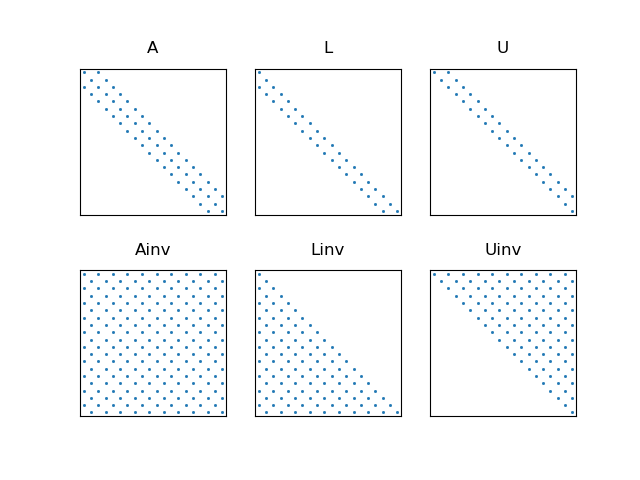
\includegraphics[width=0.8\textwidth]{figures/lu-decomposition-of-sparse-matrix}
    \item The width of the zero diagonals gets transported to the
       matrices of the LU factorization

      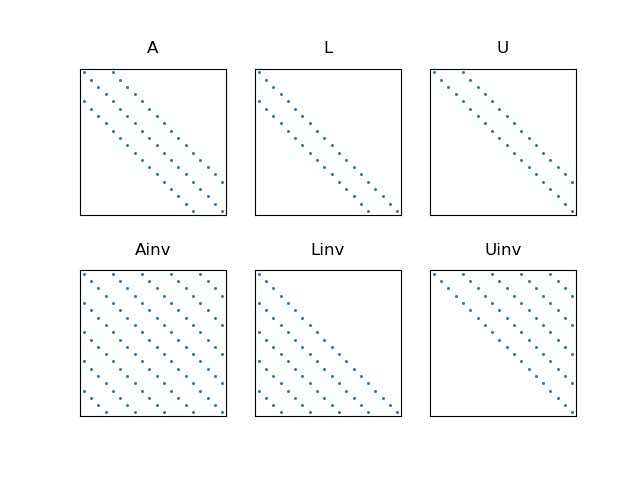
\includegraphics[width=0.8\textwidth]{figures/lu-decomposition-of-sparse-matrix-off4}
    \item The inverse is dense up to the zero diagonals that get
      scattered over the whole inverse
    \end{enumerate}

    
  \end{Solution}

  \begin{Solution}[{\cite[P-5.1 b]{Saad00}}]
    \hfill\\
    Hint 1:
    \begin{gather*}
      \scal(\mata\vd^{(k+1)},\vd^{(k+1)})
      =\scal(\mata\vd^{(k)},\vd^{(k)})
      -\frac{\scal(\vr^{(k)},\ve_i)^2}{a_{ii}}
    \end{gather*}

    Hint 2:
    \begin{gather*}
      \abs{\ve_i^T \vr^{(k)}} \geq n^{-\nfrac12}\norm{\vr^{(k)}}_2
    \end{gather*}

    With the help of hint 1 and 2 we get
    \begin{align*}
      \norm{\vd^{(k+1)}}_{\mata}^2
      = \scal(\mata\vd^{(k+1)},\vd^{(k+1)})
      &\stackrel{\text{Hint 1}}{=}
        \scal(\mata\vd^{(k)},\vd^{(k)})
        - \frac{\scal(\vr^{(k)},\ve_i)^2}{a_{ii}}
      \\
      &=
        \left( 1 - \frac{\scal(\vr^{(k)},\ve_i)^2}{a_{ii}}
              \frac1{\scal(\mata\vd^{(k)},\vd^{(k)})} \right)
        \norm{\vd^{(k)}}_{\mata}^2
      \\
      &\stackrel{\text{Hint 2}}{\leq}
        \left( 1 - \frac{1}{n a_{ii}}
              \frac{\norm{\vr^{(k)}}_2^2}{\scal(\mata\vd^{(k)},\vd^{(k)})} \right)
        \norm{\vd^{(k)}}_{\mata}^2
    \end{align*}
    The result follows by the following two estimates of Rayleigh quotients:
    \begin{gather*}
      a_{ii} = \scal(\mata\ve_i,\ve_i) = \frac{\scal(\mata\ve_i,\ve_i)}{\scal(\ve_i,\ve_i)}
      \le \lambda_{\max},
    \end{gather*}
    and
    \begin{gather*}
      \frac{\scal(\mata\vd^{(k)},\vd^{(k)})}{\norm{\vr^{(k)}}^2}
      = \frac{\scal(\vr^{(k)},\mata^{-1}\vr^{(k)})}{\norm{\vr^{(k)}}^2}
      \le \lambda_{\max}(\mata^{-1})
      = \frac1{\lambda_{\min}}.
    \end{gather*}

    Final remarks:\\
    1. Since $\ve_i\in K=L$, it holds the Galerkin-orthogonality
    \begin{align*}
      \scal(\vr^{(k)}-\alpha\mata \ve_i,\ve_i) = 0,
    \end{align*}
    where according to Example 2.3.10
    \begin{gather*}
      \alpha = \frac{\scal(\vr^{(k)},\ve_i)}{\scal(\mata\ve_i,\ve_i)}
      = \frac{\scal(\vr^{(k)},\ve_i)}{a_{ii}}
      .
    \end{gather*}
    This would have been used to show hint 1.

    2. To show hint 2, notice that by the choice of $i$ as maximal
    value of the residual vector
    \begin{align*}
      \norm{\vr^{(k)}}_2
      \leq \sqrt{n} \norm{\vr^{(k)}}_{\infty}
      = \sqrt{n} \abs{\ve_i^T\vr^{(k)}}
    \end{align*}

  \end{Solution}

  \begin{Solution}
  \end{Solution}

  \begin{Solution}[Programming]
    C++ sample code \lstinline{./programs/steepest-decent.cc} without
    assembling the system matrix.

    Convergence rate (Definition 2.2.18 in lecture notes).  As can be
    seen in the plot, the convergence of the steepest decent method is
    sublinear.

    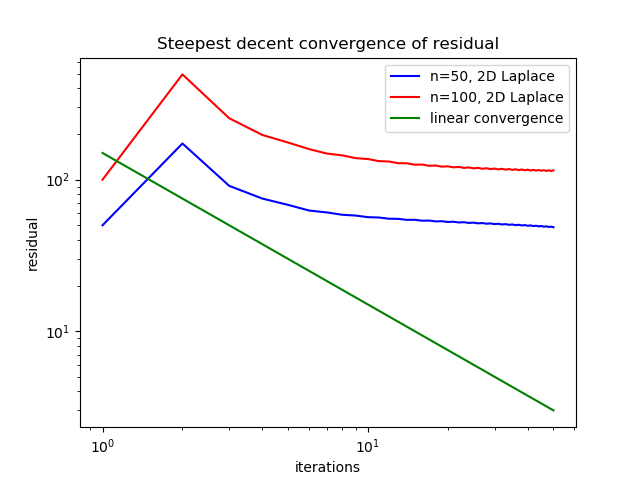
\includegraphics[width=\textwidth]{figures/laplace-steepest-decent}
  \end{Solution}

\end{SolutionSheet}


%%% Local Variables: 
%%% mode: latex
%%% TeX-master: "main"
%%% End: 

%%%%%%%%%%%%%%%%%%%%%%%%%%%%%%%%%%%%%%
% Numerical Linear Algebra class 2022 
% Sheet 9
%%%%%%%%%%%%%%%%%%%%%%%%%%%%%%%%%%%%%%

\begin{Sheet}[discussion in the first tutorials of January, 2023]
  \label{sheet9}


  This exercise sheet reviews some topics of this lecture. Your
  answers do not have to be handed in, but the exercises will be
  discussed in the tutorials of the first week of January.

  \begin{Problem}
    Recapitulate the concept of an orthogonal projection and an
    oblique projection. What are use cases of both and why are they
    important for numerical linear algebra?
  \end{Problem}

  \begin{Problem}
    What methods presented in the lecture can be used for computing or
    estimating the eigenvalues of a matrix $\mata$? Sort by properties
    of the methods, as well as by conditions on $\mata$.
  \end{Problem}

  \begin{Problem}
    How can the QR factorization of a given matrix be computed?
    Discuss downsides and benefits of the different methods.
  \end{Problem}

  \begin{Problem}
    Householder reflections vs. Givens rotations: which one is more
    cost-efficient in the general case? When using the other one is
    advantageous?
  \end{Problem}

  \begin{Problem}
    Which of the discussed methods for solving eigenvalue problems can
    be implemented without explicitly forming a matrix?
  \end{Problem}

  \begin{Problem}
    Consider an $n\times n$ matrix that has $n$ distinct eigenvalues
    such that $\abs{\lambda_i} \neq \abs{\lambda_j}$ for $i\neq
    j$. How can the eigenvalue with the second largest absolute value
    be computed?
  \end{Problem}

  \begin{Problem}
    When does one step of the Gauss-Seidel iteration provide the
    direct solution of a linear system? Consider an upper triangular
    matrix to visualize this matter.
  \end{Problem}

\end{Sheet}


%%% Local Variables: 
%%% mode: latex
%%% TeX-master: "main"
%%% End: 

%%%%%%%%%%%%%%%%%%%%%%%%%%%%%%%%%%%%%%
% Numerical Linear Algebra class 2022 
% Solutions to Sheet 9
%%%%%%%%%%%%%%%%%%%%%%%%%%%%%%%%%%%%%%

\begin{SolutionSheet}[\ref{sheet9}]
\begin{onehalfspace}

  \begin{Solution} Projection:
    \begin{itemize}
      \item $P: V \to V$ endomerphism, $P^2 = P$
      \item orthogonal $\iff \scal(Px,y) = \scal(x,Py) \iff P^2=P=P^*$ 
      (dependent on scalar product) 
      \item oblique (not orthogonal) 
      \item If $\quad W,U \subseteq V \quad W = ker(P), \ U = im(P)\\
      \implies P|_U = id_U, \\
      \phantom{\implies} V = U \oplus W$
      \item Projection Methods: Def 2.3.1, 2.3.3, Thrm 2.3.8, 2.3.9 \\
      Use cases: \begin{itemize}
        \item dimension reduction with orthogonal eigenvectors
        \item min residual Verfahren
        \item steepest descent
        \item Bestapproximation
      \end{itemize}
  \end{itemize}
  \end{Solution}

  \begin{Solution} Methods to estimate and compute eigenvalues:
    \begin{itemize}
      \item Gershgorin circles
      \item Rayleigh Quotient (Courant-Fisher) 
      \item power method
      \begin{itemize}
        \item shift
        \item inverse
      \end{itemize}
      \item QR method (Reighleigh shift, Wilkinon shift, double shift)
    \end{itemize}
  \end{Solution}

  \begin{Solution} Compute Q of the QR factorization:
    \begin{itemize}
      \item Gram-Schmidt (unstable)
      \item Householder reflection (compute from general matrix)
      \item Givens rotations (compute from Hessenberg matrix)
    \end{itemize}
  \end{Solution}

  \begin{Solution}
    See exercise 3
  \end{Solution}

  \begin{Solution}
    solving eigenvalue problems without forming the matrix: \\
    Implement function that computes the matrix vector product $Av$ for any given vector $v$ (less expensive for sparse matrices) \\
    Can be used for power method (don't need the matrix for other computations)
  \end{Solution}

  \begin{Solution}
  \end{Solution}

  \begin{Solution}
    \Claim For $A$ lower triangluar matrix, the Gauss-seidel iteration provides 
    the direct solution of the linear system $Ax=b$\\
    \Proof Let A be lower triangular \\
    $\implies A=D+L+U$ (decomp into diag, lower and upper triang) \\
    $\phantom{\implies}$where $U = 0, \ L+D = A\\
    \\
    \stackrel{Lemma \ 2.2.5}{\implies}$ Gauss-Seidel:
    \begin{align*}
      x^{k+1} &= (\I - (D+L)^{-1} A) x^k + (D+L)^{-1} b \\
       &= (\I - A^{-1} A) x^k + A^{-1} b \\
       &= A^{-1}b
    \end{align*}
  \end{Solution}

\end{onehalfspace}
\end{SolutionSheet}


%%% Local Variables: 
%%% mode: latex
%%% TeX-master: "main"
%%% End: 

%%%%%%%%%%%%%%%%%%%%%%%%%%%%%%%%%%%%%%
% Numerical Linear Algebra class 2022 
% Sheet 10
%%%%%%%%%%%%%%%%%%%%%%%%%%%%%%%%%%%%%%

\begin{Sheet}[to be handed in until January 20, 2023, 2pm.]
  \label{sheet10}

  \begin{Problem}[{\cite[Exercise 6.21]{Saad00}}]
    % Saad Aufgabe 21 (S. 214)
    Consider a matrix of the form:
    \begin{gather*}
      \mata = \id + \alpha \matb
    \end{gather*}
    where $\matb$ is skew-symmetric (real), that is,
    $\matb^T = -\matb$.
    \begin{enumerate}[(a)]
    \item Show that
      \begin{gather*}
        \frac{\scal(\mata\vx,\vx)}{\scal(\vx,\vx)} = 1
      \end{gather*}
      for all nonzero $\vx$.
    \item\label{sheet10:problem1:partb} Consider the Arnoldi process
      for $\mata$. Show that the resulting Hessenberg matrix will have
      the following tridiagonal form
      \begin{gather*}
        \matH_m =
        \begin{pmatrix}
          1&-\eta_2&&& \\
          \eta_2&1&-\eta_3&& \\
           &\ddots&\ddots&\ddots& \\
           &&\eta_{m-1}&1&-\eta_m \\
           &&&\eta_m&1
        \end{pmatrix}
        .
      \end{gather*}
    \item Using the result of part \eqref{sheet10:problem1:partb},
      explain why the conjugate gradient method applied to a linear
      system with the matrix $\mata$ will still yield residual vectors
      that are orthogonal to each other.
    \item Can this algorithm break down before the solution is
      reached?
    \end{enumerate}
  \end{Problem}

  \begin{Problem}[{\cite[Exercise 6.8]{Saad00}}]
    Show how GMRES (Algorithm 2.3.41 in the lecture notes) and Arnoldi
    with modified Gram-Schmidt (Algorithm 2.3.29 in the lecture notes)
    will converge on the linear system $\mata\vx=\vb$ when
    \begin{gather*}
      \mata =
      \begin{pmatrix}
        &&&&1\\
        1&&&&\\
        &1&&&\\
        &&1&&\\
        &&&1&
      \end{pmatrix},
      \quad
      \vb =
      \begin{pmatrix}
        1\\ 0\\ 0\\ 0\\ 0
      \end{pmatrix},
    \end{gather*}
    and $\vx_0 = \boldsymbol 0$.
  \end{Problem}

  \begin{Problem}[Programming]
    \hfill\\\vspace{-4ex}
    \begin{enumerate}[(a)]
    \item Implement the conjugate gradient method (Algorithm 2.3.57 in
      the lecture notes).
    \item Use your implementation to solve the 2D Laplace problem
      \begin{gather*}
        \matl_2\vx=\vb
      \end{gather*}
      as in \cref{sheet7:problem4} on \cref{sheet7} with right hand
      side vector $\vb=(1,...,1)^T$ and initial guess
      $\vx^{(0)}=(0,...,0)^T$ with $n=50$ and $n=100$. Observe the
      convergence for the first 50 steps. What convergence rate do you
      expect? Compare your results of the conjugate gradient method
      with the steepest decent method from \cref{sheet8:problem4} of
      \cref{sheet8}.
    \end{enumerate}
  \end{Problem}

  \vfill
  \bibliographystyle{alpha}
  \bibliography{bib}
\end{Sheet}


%%% Local Variables: 
%%% mode: latex
%%% TeX-master: "main"
%%% End: 

%%%%%%%%%%%%%%%%%%%%%%%%%%%%%%%%%%%%%%
% Numerical Linear Algebra class 2022 
% Solutions to Sheet 10
%%%%%%%%%%%%%%%%%%%%%%%%%%%%%%%%%%%%%%

\begin{SolutionSheet}[\ref{sheet10}]

  \begin{Solution}
  \end{Solution}

  \begin{Solution}
  \end{Solution}

  \begin{Solution}
  \end{Solution}

  \begin{Solution}[Programming]
  \end{Solution}

\end{SolutionSheet}


%%% Local Variables: 
%%% mode: latex
%%% TeX-master: "main"
%%% End: 

\end{document}


%%% Local Variables: 
%%% mode: latex
%%% TeX-master: "main"
%%% End: 
